\chapter{设备树(DTS)}
设备树是什么?又为何要引入设备树呢?这个需要追溯到2011年3月17日。这天
Linus Torvalds对ARM Linux邮件列表宣称“this whole ARM thing is a fucking pain in the 
ass”,ARM Linux社区对此作出了回应,由此引入设备树。在未引入设备树之前,Linux源码中充斥这非常多的驱动
代码,这些驱动代码虽然完整的适应很多处理器架构,但是由于处理器种类太多,而且每种处理器又分了非常多不同型号
的处理器,这使得相应的驱动文件异常的多,Linus称其为垃圾代码。其后,Linux源码开始引入设备树,将不同型号的
处理器驱动尽可能放在一起,为了方便管理,他们将所有的设备都描述成一棵树,Linux内核启动之后就会遍历这颗树,
然后初始化相应的硬件。在设备树引入之前,Platform总线也是非常好的一个设备驱动框架,读者有兴趣可以深入了解,
这种框架当前任然还保留在,而且当前几乎大部分驱动都是Platform总线结合设备树一起管理驱动设备。


在Linux发展过程中总共经历了三种设备驱动管理框架,第一种是最原始的基于简单的注册,这种方式比较容易理解,需
要什么设备驱动就将相应的驱动写在内核中,然后编译即可载入内核。这种方法缺陷很明显,当设备越来越多时,驱动文
件将变得很大。最后PowerPC使用了一种基于Platform Bus的框架,这种框架改善的上面的情况,它将处理器虚与设备之
间的交互虚拟成一根总线,相同类型的驱动使用同一根总线,比如IIC,IIS,SPI,USB等等,所有的设备都是这些总线上的
子设备。第三种就是现在的基于设备树的驱动框架,这种驱动框架结合了Platform 
Bus的优点,同时引入了设备树概念,其核心思想是将处理器看作是一个数的主干,主干上有很多分支,分支上挂载着不
同的设备。


需要说明的是设备树并不是驱动文件,它指示一个描述设备的表格,而真是的驱动代码会根据设备树选择的设备对相应的
设备进行初始化,设备树上没有的设备不会初始化。这举个简单的例子:现在我们需要对两个数进行四则运算,但是我们
暂时不知道具体是哪一种运算,那我们就可以这样写
\begin{lstlisting}[language={[ANSI]C},numbers=left,numberstyle=\tiny,frame=shadowbox,
		rulesepcolor=\color{red!20!green!20!blue!20},
		keywordstyle=\color{blue!70!black},
		commentstyle=\color{blue!90!},
		basicstyle=\ttfamily]
		int fun(int style,int x,int y)
		{
			switch(style)
			{
				case 0:return x+y;
				case 1:return x-y;
				case 2:return x*y;
				case 3:return x/y;
				default:return -1;
			}
		}
\end{lstlisting}
如果要进行四则运算,dts可以看作是选择其中一个运算方式。
\begin{figure}[h]
	\centering
	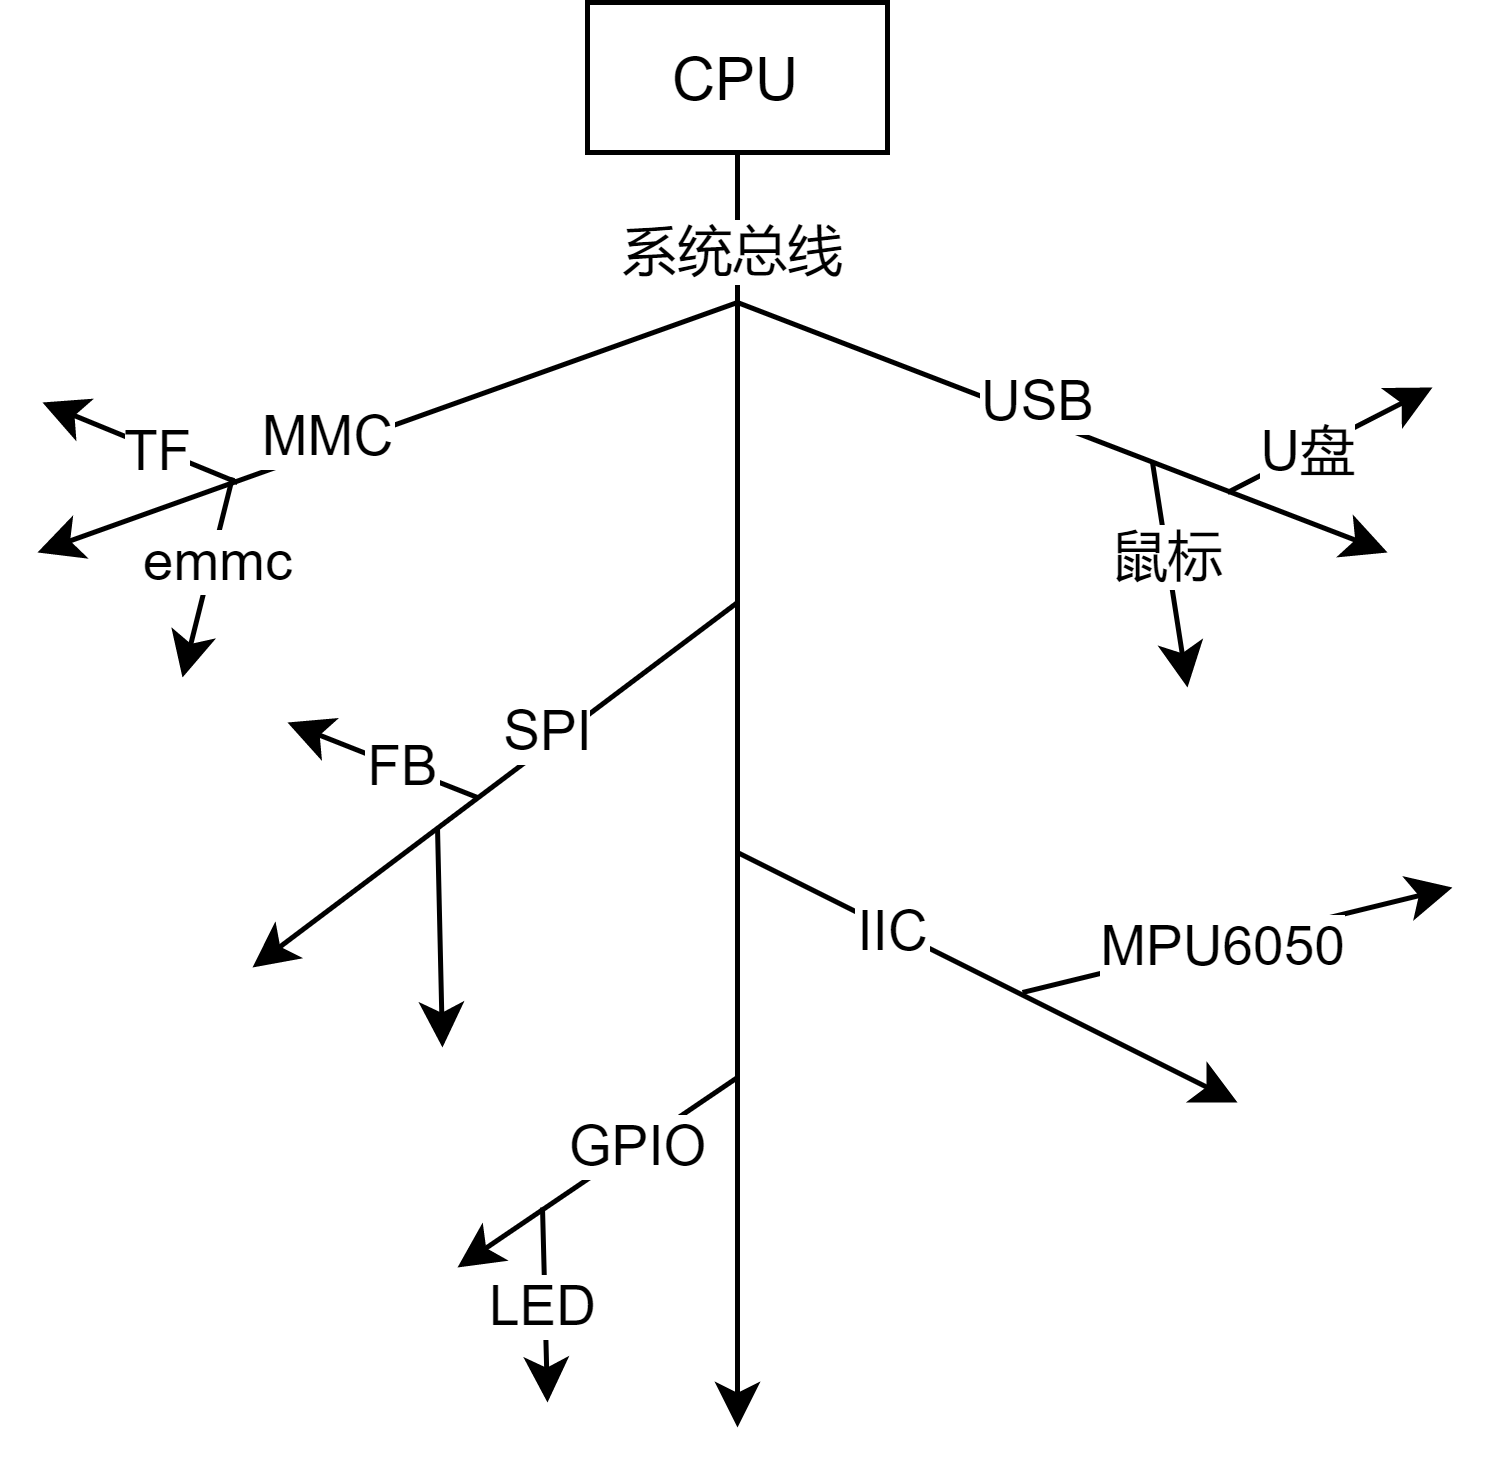
\includegraphics[width=1\linewidth]{chapter3/img/DTS}
	\caption{}
	\label{fig:dts}
\end{figure}
图\ref{fig:dts}所示是dts的示意图,可以看到每个设备都是通过总线的方式描述的。
\begin{figure}[htbp]
	\centering
	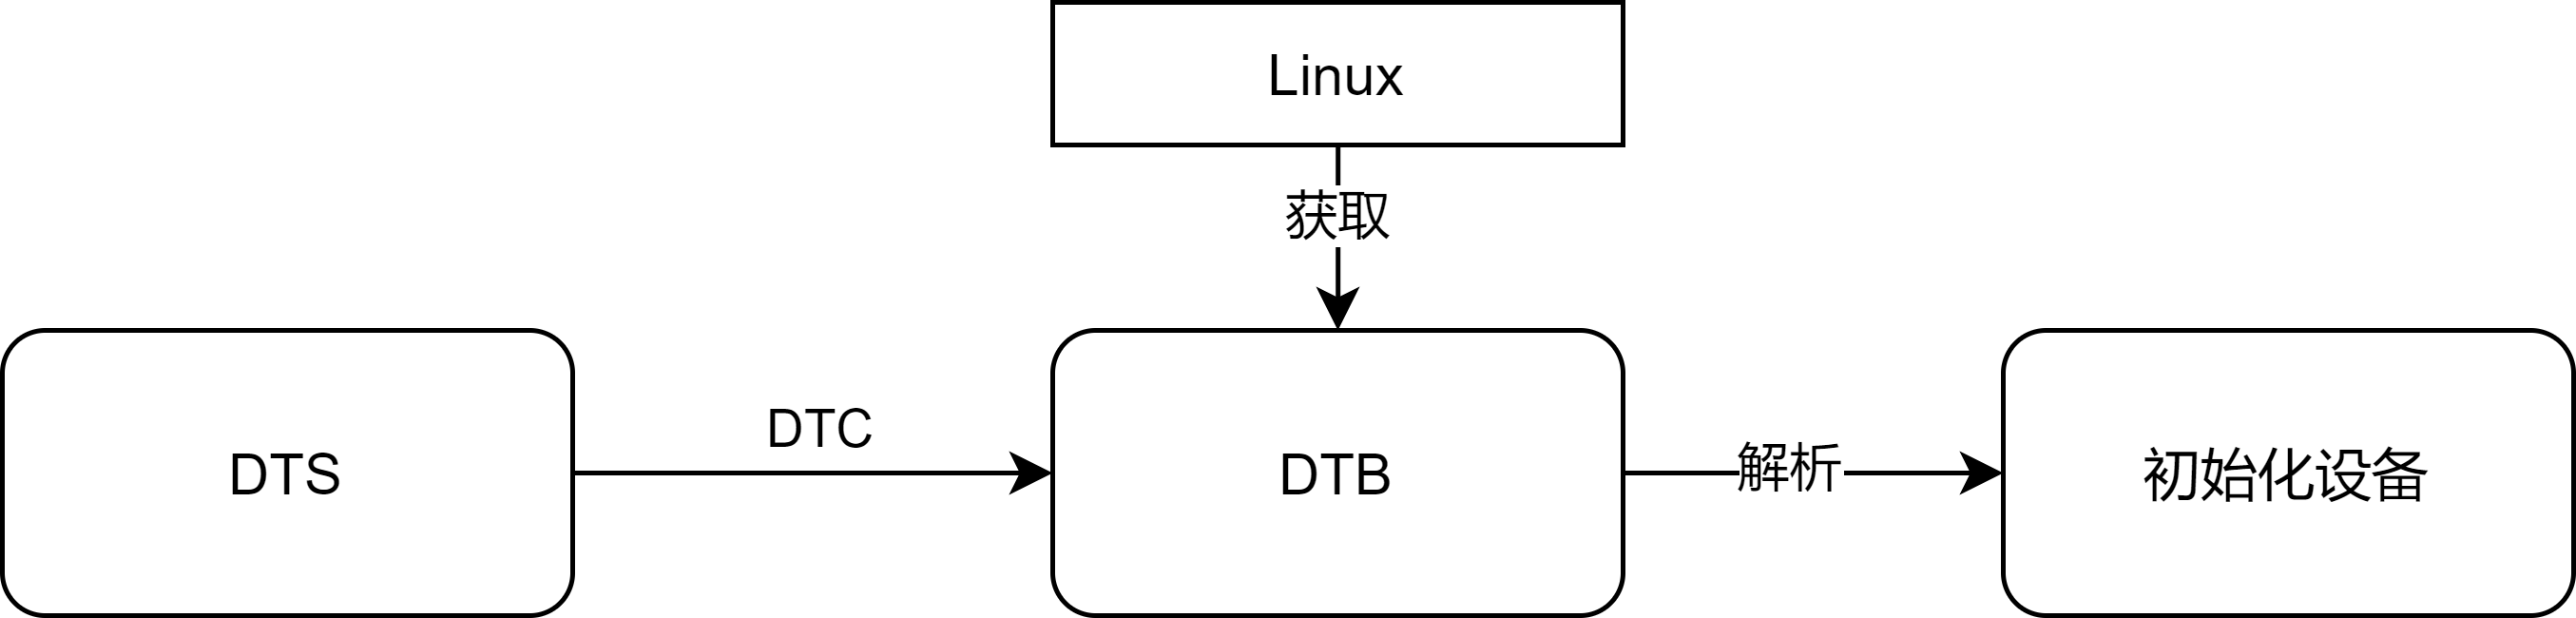
\includegraphics[width=0.6\linewidth]{chapter3/img/DTSstream}
	\caption{}
	\label{fig:dtsstream}
\end{figure}
图\ref{fig:dtsstream},dts文件需要被dtc编译器编译为dtb的二进制文件,当内核获取dtb文件后会对文件进行解析,
然后根据dtb文件的内容对相应的设备进行初始化以及注册。
\begin{tcolorbox}[colback=red!5!white,colframe=red!75!black]
	\faWarning\  
	一般而言,dts会分为两个文件,一个是dtsi文件,另一个是dts文件。dtsi文件类似于.h文件一样,dts文件一般包
	含dtsi文件,然后根据需要来配置设备节点。
\end{tcolorbox}

\section{dts文件结构}
先来看下suniv-f1c100s的dtsi文件,打开Linux5.7源码中的arch/arm/boot/dts/suniv-f1c100s.dtsi文件

\begin{lstlisting}[language={[ANSI]C},numbers=left,numberstyle=\tiny,frame=shadowbox,
	rulesepcolor=\color{red!20!green!20!blue!20},
	keywordstyle=\color{blue!70!black},
	commentstyle=\color{blue!90!},
	basicstyle=\ttfamily]
	#include <dt-bindings/clock/suniv-ccu-f1c100s.h>
	#include <dt-bindings/reset/suniv-ccu-f1c100s.h>
	/ {
		#address-cells = <1>;
		#size-cells = <1>;
		interrupt-parent = <&intc>;
		clocks {
			osc24M: clk-24M {
				#clock-cells = <0>;
				compatible = "fixed-clock";
				clock-frequency = <24000000>;
				clock-output-names = "osc24M";
			};
			
			osc32k: clk-32k {
				#clock-cells = <0>;
				compatible = "fixed-clock";
				clock-frequency = <32768>;
				clock-output-names = "osc32k";
			};
		};
		
		cpus {
			cpu {
				compatible = "arm,arm926ej-s";
				device_type = "cpu";
			};
		};
		
		soc {
			compatible = "simple-bus";
			#address-cells = <1>;
			#size-cells = <1>;
			ranges;
			
			sram-controller@1c00000 {
				compatible = "allwinner,suniv-f1c100s-system-control",
				"allwinner,sun4i-a10-system-control";
				reg = <0x01c00000 0x30>;
				#address-cells = <1>;
				#size-cells = <1>;
				ranges;
				
				sram_d: sram@10000 {
					compatible = "mmio-sram";
					reg = <0x00010000 0x1000>;
					#address-cells = <1>;
					#size-cells = <1>;
					ranges = <0 0x00010000 0x1000>;
					
					otg_sram: sram-section@0 {
						compatible = "allwinner,suniv-f1c100s-sram-d",
						"allwinner,sun4i-a10-sram-d";
						reg = <0x0000 0x1000>;
						status = "disabled";
					};
				};
			};
			
			ccu: clock@1c20000 {
				compatible = "allwinner,suniv-f1c100s-ccu";
				reg = <0x01c20000 0x400>;
				clocks = <&osc24M>, <&osc32k>;
				clock-names = "hosc", "losc";
				#clock-cells = <1>;
				#reset-cells = <1>;
			};
		};
	};
\end{lstlisting}
由于文件太大,上面的dtsi文件只放一部分,可以看到里面有很多关于设备的描述信息,下面将重点讲解其意义。
1-2行是包含的头文件,该头文件中定义了时钟宏和复位相关的宏,这些宏可以在dtsi和dts文件中看到,例如osc24M等,
这两个头文件在include/dt-bindings/clock和include/dt-bindings/reset目录里面。

一般默认规定,dtsi文件放一个系列芯片的公共部分,然后dts文件对其节点进行配置。F1C200S的dtsi文件中说明了几
乎所有的硬件描述,dts文件中对各个硬件节点进行配置。这样对于不同开发板而言,只需要编写dts文件即可完成配置,
当然,前提是dtsi文件中的硬件描述是完整的。
\subsection{节点}
所谓节点是针对总线而言的,将根节点作为一个树的根,然后在根节点上添加其他的节点。上述给的dtsi文件中/就是根
节点,根节点里面会添加各个其他的不同节点,对于一个dts文件而言,有且只有一个根节点。
从上面可以看到有些节点前面有:,例如clock节点:
\begin{lstlisting}[language={[ANSI]C},numbers=left,numberstyle=\tiny,frame=shadowbox,
	rulesepcolor=\color{red!20!green!20!blue!20},
	keywordstyle=\color{blue!70!black},
	commentstyle=\color{blue!90!},
	basicstyle=\ttfamily]
	ccu: clock@1c20000 {
		compatible = "allwinner,suniv-f1c100s-ccu";
		reg = <0x01c20000 0x400>;
		clocks = <&osc24M>, <&osc32k>;
		clock-names = "hosc", "losc";
		#clock-cells = <1>;
		#reset-cells = <1>;
	};
\end{lstlisting}
该节点的节点名为clock,地址为0x1c20000,因此,节点的表示为:节点名\&地址。
\begin{tcolorbox}[colback=red!5!white,colframe=red!75!black]
	\faWarning\
	这里的节点名@后面的地址并不是真实的地址,可以随便写一个,但是为了不发生重复,一般默认规定其值为该寄存
	器的地址。只有reg属性中的地址才是真实描述寄存器的地址。
\end{tcolorbox}
这里的ccu是一个节点标号,所谓节点标号可以看作是该节点的一个别名,这样做的好处是当需要修改节点的属性时,只
需要在dts文件中引用该标号,然后添加修改的属性即可,而不需要重复将该节点完整的写一遍。例如现在需要将ccu节点
中的属性clocks修改为<\&osc32M>, <\&osc32.768>;,此时只需要在dts文件中这样写即可:
\begin{lstlisting}[language={[ANSI]C},numbers=left,numberstyle=\tiny,frame=shadowbox,
	rulesepcolor=\color{red!20!green!20!blue!20},
	keywordstyle=\color{blue!70!black},
	commentstyle=\color{blue!90!},
	basicstyle=\ttfamily]
	&ccu{
		clocks = <&osc32M>, <&osc32.768k>;
	};
\end{lstlisting}
\begin{note}
	一般需要修改节点的status属性以及引脚属性。
\end{note}
\subsection{属性}
每个节点必须要有属性,所谓属性就是添加一些节点的必要信息,比如寄存器地址,时钟等,这些属性是为驱动程序提供
具体的相关信息的,下面来简单讲解下一般接触到的节点属性。


\subsubsection{compatible}
"compatible"表示“兼容”,对于某个LED,内核中可能有A、B、C三个驱动都支持它,那可以这样写:\\
led\{compatible = "A", "B", "C";\};  \\
内核启动时,就会为这个LED按这样的优先顺序为它找到驱动程序:A、B、C。
也可以从上面的clock节点可以看到其兼容属性为\\
compatible = "allwinner,suniv-f1c100s-ccu";\\
内核会通过of\_match\_table(也有通过of\_find\_compatible\_node)来匹配对应的节点,一旦匹配到就加载该驱动
。因此当前大部分的驱动都需要使用compatible
节点来加载驱动程序,以降低不必要的代码量。有这么一个默认的规定,compatible后面一般格式为“厂家,驱动名称”,
这只是一个约定俗称的规定,不一定非要这样写,只要驱动程序能够与dts文件中的节点属性对应起来就可以。对于有些
节点可以兼容多个设备时,可以写在一起,例如:\\
compatible = "allwinner,suniv-f1c100s-ccu","allwinner,suniv-f1c200s-ccu";

\subsubsection{model}
"model"字面意思是模型,主要来说明该设备的具体名称,例如上面我们可以添加一个model属性:\\
\begin{lstlisting}[language={[ANSI]C},numbers=left,numberstyle=\tiny,frame=shadowbox,
	rulesepcolor=\color{red!20!green!20!blue!20},
	keywordstyle=\color{blue!70!black},
	commentstyle=\color{blue!90!},
	basicstyle=\ttfamily]
	ccu: clock@1c20000 {
		compatible = "allwinner,suniv-f1c100s-ccu";
		model = "lite200";
		reg = <0x01c20000 0x400>;
		clocks = <&osc24M>, <&osc32k>;
		clock-names = "hosc", "losc";
		#clock-cells = <1>;
		#reset-cells = <1>;
	};
\end{lstlisting}
上面添加了一个model = "lite200";属性来说明此设备是lite200,一般而言,此驱动会被加载打印出来,不过并不是
必须的,也可以没有此属性。

\subsubsection{status}
"status"可以看出这个属性是状态的意思,在dts节点中表示此节点是否有效,其属性有
\begin{table}[htbp]
	\centering
	\caption{status属性值}
	\begin{tabular}{ccccccc}
	\hline
	okay & 表示设备可操作 \\
	\hline
	disabled & 表示设备不可操作 \\
	\hline
	fail & 表示设备不可操作,同时检测到设备错误   \\
	\hline
	fail-sss & 表示设备不可操作,同时检测到sss错误  \\
	\hline
\end{tabular}
\end{table}
大多数情况下接触的只有okay和disable这两个属性。

\subsubsection{ \#address-cells \  \#size-cells}
address-cells表示该节点的地址要用多少个32位数来表示,size-cells表示该节点的大小要用多少个32位数来表示。
这两个属性与后面的reg属性比较密切,因为reg属性需要用这两个属性来说明其寄存器所占用的空间大小。例如:
\begin{lstlisting}[language={[ANSI]C},numbers=left,numberstyle=\tiny,frame=shadowbox,
	rulesepcolor=\color{red!20!green!20!blue!20},
	keywordstyle=\color{blue!70!black},
	commentstyle=\color{blue!90!},
	basicstyle=\ttfamily]
	sram_d: sram@10000 {
		compatible = "mmio-sram";
		reg = <0x00010000 0x1000>;
		#address-cells = <1>;
		#size-cells = <1>;
		ranges = <0 0x00010000 0x1000>;
		
		otg_sram: sram-section@0 {
			compatible = "allwinner,suniv-f1c100s-sram-d",
			"allwinner,sun4i-a10-sram-d";
			reg = <0x0000 0x1000>;
			status = "disabled";
		};
	};
\end{lstlisting}
上面的\\
\#address-cells = <1>;\\
\#size-cells = <1>;\\
这两个表示reg的地址占一个32位数,即4个字节,大小占一个32位数,即4个字节。这样就可以清楚的知道reg = 
<0x00010000 0x1000>;的意思是寄存器的地址位0x00010000,大小为0x1000。

\begin{tcolorbox}[colback=red!5!white,colframe=red!75!black]
	\faWarning\  
	\#address-cells和\#size-cells属性不是从devicetree的祖先继承的。它们需要明确定义,如果未定义,对于设
	备树则默认按照地址cell为2个,长度cell为1个去解析reg的值。
\end{tcolorbox}







\subsubsection{reg}
这个属性表示寄存器的地址,这个属性非常重要,因为设备驱动最重操作的是寄存器的值。在加载内核驱动后,内核首先
要做的是解析DTB文件,通过获取DTB文件就可以获取设备相应的寄存器地址。在设备树中,reg属性是描述一段内存的,
这段内存的大小由\#address-cells和\#size-cells决定,其中\#address-cells表示设备树总线宽度需要用多少个cell
表示(默认一个cell为32位,即四个字节),\#size-cells表示设备树总线上设备挂载的地址空间大小需要多少个cell表
示。






\subsubsection{ranges}
该属性一般为空,如果不为空,则表示一个地址映射表或者叫地址转换表,其一般








\section{设备树与驱动关系}






